% Template for articles for CCR (Computational Communication Research)

% This file contains information such as author, title, etc.
% Edit the body.tex file to add the contents (or change the % The article body
% Also see main.tex for information such as authors, title, etc
% See https://www.overleaf.com/learn/ for some great resources on learning latex

\section{Introdução}

Trabalho desenvolvido a partir de dados coletados em laboratório no dia 14 de fevereiro de 2023, contendo analise a resolução de questionário sobre o experimento Região Proibida do Germânio.

\section{Questionário}
\subsection{Explique o que é um semicondutor intrínseco e extrínseco?}
Semicondutores são materiais com condutividade elétrica intermediária entre condutores e isolantes. Existem dois tipos de semicondutores: intrínsecos e extrínsecos. Os semicondutores intrínsecos são materiais puros como o silício e o germânio, enquanto os extrínsecos são materiais dopados com pequenas quantidades de outros elementos químicos para alterar suas propriedades elétricas. A compreensão da diferença entre os semicondutores intrínsecos e extrínsecos é essencial para entender a variação da condutividade elétrica nesses materiais e, consequentemente, para o desenvolvimento de tecnologias eletrônicas avançadas.

\subsection{Mostre como obter a equação (1.1) do roteiro.}

 \begin{equation}  \sigma = \frac{1}{\rho} \label{eq1}\end{equation}
 \begin{equation} R = \frac{V}{I} = \rho \cdot \frac{L}{A} \label{eq2}\end{equation}
\begin{equation} \frac{V}{I} =\frac{1}{\sigma} \cdot \frac{L}{A}\label{eq3}\end{equation}
 \begin{equation} \sigma = \frac{I \cdot L}{V\cdot A} \left[\frac{1}{\Omega\cdot m}\right]\label{eq4}\end{equation}
 Onde,  $\sigma =$ condutividade intrínseca$\left [ {\left(\Omega\cdot m\right)}^{-1} \right ]$; $L=$ comprimento $\left[m\right]$, $A=$ area da seção transversal $\left[m^2\right]$; $V=$ tensão elétrica $\left[V\right]$ e $I=$ corrente elétrica $\left[A\right]$.


\subsection{Calcule a condutividade intrínseca do germânio a temperatura ambiente.}
Utilizando um valor de tensão no momento em que a temperatura é equivalente a ambiente temos:
\begin{equation} \sigma_{amb} =\frac{I \cdot L}{V(T_{amb})\cdot A} \label{eq5}\end{equation}
\begin{equation} \sigma_{amb} =\frac{0,005 \cdot 0,02}{4,28\cdot 0,01\cdot 0,001} \label{eq6}\end{equation}
\begin{equation} \sigma_{amb} =2,336\left[\frac{1}{\Omega\cdot m}\right] \label{eq7}\end{equation}

\subsection{Faça o gráfico condutividade \texorpdfstring{$\sigma$ x $T$}{} para o germânio intrínseco.}
    \begin{figure}[H]
        \centering    
        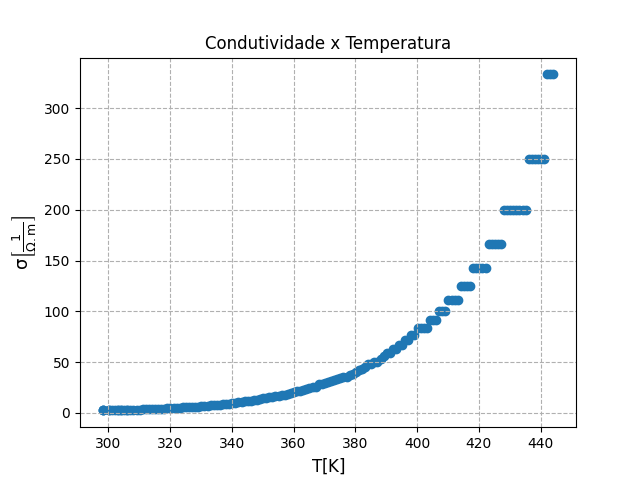
\includegraphics[width = \textwidth]{Figure_1.png}\label{fig1}
        \caption{Gráfico de condutividade intrínseca do germânio por temperatura}
    \end{figure}


\subsection{Faça o gráfico condutividade \texorpdfstring{$\ln \sigma$ x $T^{-1}$}{} para o germânio intrínseco.}
\begin{figure}[H]   
        \centering
        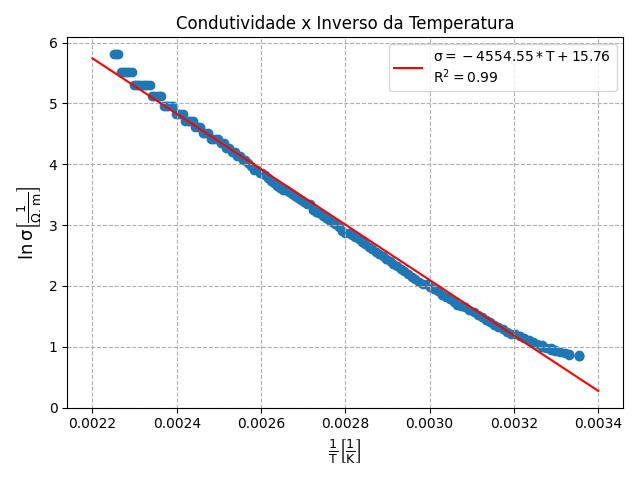
\includegraphics[width = \textwidth]{Figure_2.png}\label{fig2}
        \caption{Log natural da condutividade intrínseca do germânio por inverso da temperatura}
    \end{figure}


\subsection{Calcule o valor do coeficiente angular o gráfico acima. Qual é o significado físico do coeficiente angular do gráfico \texorpdfstring{$\ln \sigma$ x $T^{-1}$?}{}}
Partindo da regressão linear, tem que o coeficiente angular é igual à -4554,55.


\subsection{Calcule o valor obtido da energia de região proibida do germânio a partir do gráfico acima e compare com o teórico.}
Dado que:
\begin{equation} \sigma = \sigma_{0}\cdot\exp\left({-\frac{Eg}{2\cdot k \cdot T}}\right)
\label{eq8}\end{equation}
\begin{equation} \ln\sigma = \ln\sigma_{0} + \ln\left[\exp\left({-\frac{Eg}{2\cdot k \cdot T}}\right)\right] \label{eq9}\end{equation}
\begin{equation} \ln\sigma = -\frac{Eg}{2\cdot k \cdot T} + \ln\sigma_{0} \label{eq10}\end{equation}
\begin{equation} \ln\sigma = \frac{\alpha}{T} + \ln\sigma_{0} \label{eq11}\end{equation}

\begin{equation} -\frac{Eg}{2\cdot k } =  \alpha \label{eq12}\end{equation}
\begin{equation} Eg = -2\cdot \alpha \cdot k \label{eq13}\end{equation}
\begin{equation} Eg = -2\cdot (-4554,55) \cdot 8,62 \cdot 10^{-5} \label{eq14}\end{equation}
\begin{equation} Eg = 0,78 \left[eV\right] \label{eq15}\end{equation}

Onde: $Eg$ = Energia da região proibida $\left[eV\right]$, $\alpha =$ coeficiente angular da linearização dos dados de condutividade, $T=$ temperatura $\left[K\right]$, $k=$ constante de Boltzmann; que é igual à $8,62 \cdot 10^{-5}  \left[k/eV\right]$
\newpage
\subsection{Dados}

\begin{table}[h!]
    \footnotesize
    \caption{Dados coletados}      
    \begin{tabular}{|c|c|c|c|c|c|c|c|c|c|c|c|}
    \hline
    \multicolumn{12}{|c|}{Dados coletados em lab}\\
    \hline
$^{\circ}C$&$Vp$&$K$&$^{\circ}C$&$Vp$&$K$&$^{\circ}C$&$Vp$&$K$&$^{\circ}C$&$Vp$&$K$
    \csvreader[]{dadoslatex.csv}{1=\CC, 2=\VV, 3=\KK, 4=\CCC, 5=\VVV, 6=\KKK, 7=\CCCC, 8=\VVVV, 9=\KKKK, 10=\CCCCC, 11=\VVVVV, 12=\KKKKK}{\\ \hline \CC&\VV&\KK&\CCC&\VVV&\KKK&\CCCC&\VVVV&\KKKK&\CCCCC&\VVVVV&\KKKKK} \\
    \hline
    
    \end{tabular}
    \label{tabela}
    
\end{table}



  

 below)

\documentclass{ccr}
\usepackage{amsmath}
\usepackage{etoolbox}
\usepackage{mathtools}
\numberwithin{equation}{subsection}
\usepackage{caption}
\usepackage{float}
\usepackage{csvsimple,longtable,booktabs}
\usepackage{graphicx}

% Note - lines starting with a % are completely ignored by latex and function as comments
% See https://www.overleaf.com/read/hmwdsgcqkxrd for a complete example article

% The first part of the latex document contains metadata

% Regular metadata (title, authors etc)
\title{Atividade II}
\authorsnames{Daniel Florencio de Aquino Faria}
% Short author list for footer


% Note that you need to provide as many affiliations as authors
% If multiple authors have the same affiliation, please copy that record as needed
\authorsaffiliations{
  {Universidade Federal do ABC}, 
}

% You can add or rename the bibliography file(s) here
% Note that you can exported them from endnote or zotero directly and upload them to overleaf
\addbibresource{bibliography.bib}


% The following information is provided by the journal when moving to production


% some packages that are generally useful when writing articles in latex
\usepackage{tabularx}  % for full-width tables
\usepackage{booktabs}  % for nicer horizontal lines in tables
\usepackage[mode=text]{siunitx} % for centering columns on the decimal mark
\usepackage{graphicx} % for including figures
\usepackage{csquotes}\MakeOuterQuote{"}  % to allow "double quotes" instead of ``double quote''
\usepackage[hidelinks]{hyperref} % for URLs and other hyperlinks


\begin{document}
\maketitle

% The article body
% Also see main.tex for information such as authors, title, etc
% See https://www.overleaf.com/learn/ for some great resources on learning latex

\section{Introdução}

Trabalho desenvolvido a partir de dados coletados em laboratório no dia 14 de fevereiro de 2023, contendo analise a resolução de questionário sobre o experimento Região Proibida do Germânio.

\section{Questionário}
\subsection{Explique o que é um semicondutor intrínseco e extrínseco?}
Semicondutores são materiais com condutividade elétrica intermediária entre condutores e isolantes. Existem dois tipos de semicondutores: intrínsecos e extrínsecos. Os semicondutores intrínsecos são materiais puros como o silício e o germânio, enquanto os extrínsecos são materiais dopados com pequenas quantidades de outros elementos químicos para alterar suas propriedades elétricas. A compreensão da diferença entre os semicondutores intrínsecos e extrínsecos é essencial para entender a variação da condutividade elétrica nesses materiais e, consequentemente, para o desenvolvimento de tecnologias eletrônicas avançadas.

\subsection{Mostre como obter a equação (1.1) do roteiro.}

 \begin{equation}  \sigma = \frac{1}{\rho} \label{eq1}\end{equation}
 \begin{equation} R = \frac{V}{I} = \rho \cdot \frac{L}{A} \label{eq2}\end{equation}
\begin{equation} \frac{V}{I} =\frac{1}{\sigma} \cdot \frac{L}{A}\label{eq3}\end{equation}
 \begin{equation} \sigma = \frac{I \cdot L}{V\cdot A} \left[\frac{1}{\Omega\cdot m}\right]\label{eq4}\end{equation}
 Onde,  $\sigma =$ condutividade intrínseca$\left [ {\left(\Omega\cdot m\right)}^{-1} \right ]$; $L=$ comprimento $\left[m\right]$, $A=$ area da seção transversal $\left[m^2\right]$; $V=$ tensão elétrica $\left[V\right]$ e $I=$ corrente elétrica $\left[A\right]$.


\subsection{Calcule a condutividade intrínseca do germânio a temperatura ambiente.}
Utilizando um valor de tensão no momento em que a temperatura é equivalente a ambiente temos:
\begin{equation} \sigma_{amb} =\frac{I \cdot L}{V(T_{amb})\cdot A} \label{eq5}\end{equation}
\begin{equation} \sigma_{amb} =\frac{0,005 \cdot 0,02}{4,28\cdot 0,01\cdot 0,001} \label{eq6}\end{equation}
\begin{equation} \sigma_{amb} =2,336\left[\frac{1}{\Omega\cdot m}\right] \label{eq7}\end{equation}

\subsection{Faça o gráfico condutividade \texorpdfstring{$\sigma$ x $T$}{} para o germânio intrínseco.}
    \begin{figure}[H]
        \centering    
        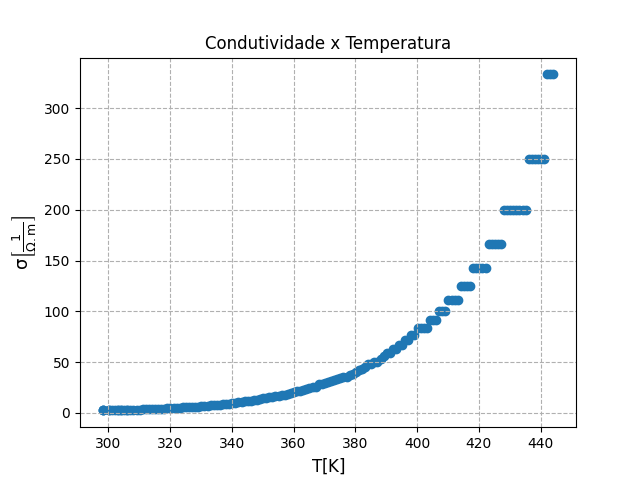
\includegraphics[width = \textwidth]{Figure_1.png}\label{fig1}
        \caption{Gráfico de condutividade intrínseca do germânio por temperatura}
    \end{figure}


\subsection{Faça o gráfico condutividade \texorpdfstring{$\ln \sigma$ x $T^{-1}$}{} para o germânio intrínseco.}
\begin{figure}[H]   
        \centering
        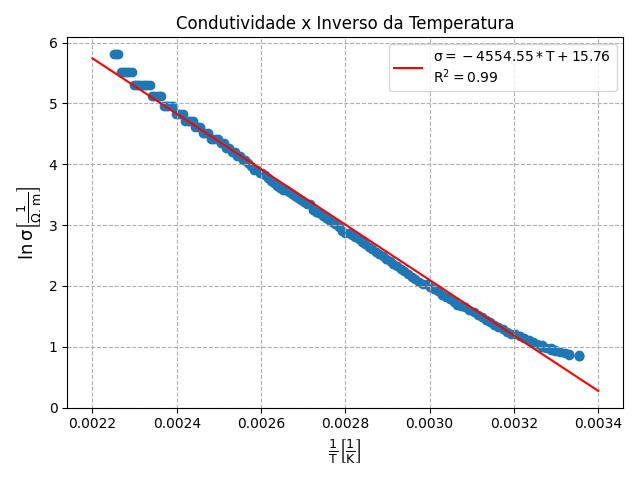
\includegraphics[width = \textwidth]{Figure_2.png}\label{fig2}
        \caption{Log natural da condutividade intrínseca do germânio por inverso da temperatura}
    \end{figure}


\subsection{Calcule o valor do coeficiente angular o gráfico acima. Qual é o significado físico do coeficiente angular do gráfico \texorpdfstring{$\ln \sigma$ x $T^{-1}$?}{}}
Partindo da regressão linear, tem que o coeficiente angular é igual à -4554,55.


\subsection{Calcule o valor obtido da energia de região proibida do germânio a partir do gráfico acima e compare com o teórico.}
Dado que:
\begin{equation} \sigma = \sigma_{0}\cdot\exp\left({-\frac{Eg}{2\cdot k \cdot T}}\right)
\label{eq8}\end{equation}
\begin{equation} \ln\sigma = \ln\sigma_{0} + \ln\left[\exp\left({-\frac{Eg}{2\cdot k \cdot T}}\right)\right] \label{eq9}\end{equation}
\begin{equation} \ln\sigma = -\frac{Eg}{2\cdot k \cdot T} + \ln\sigma_{0} \label{eq10}\end{equation}
\begin{equation} \ln\sigma = \frac{\alpha}{T} + \ln\sigma_{0} \label{eq11}\end{equation}

\begin{equation} -\frac{Eg}{2\cdot k } =  \alpha \label{eq12}\end{equation}
\begin{equation} Eg = -2\cdot \alpha \cdot k \label{eq13}\end{equation}
\begin{equation} Eg = -2\cdot (-4554,55) \cdot 8,62 \cdot 10^{-5} \label{eq14}\end{equation}
\begin{equation} Eg = 0,78 \left[eV\right] \label{eq15}\end{equation}

Onde: $Eg$ = Energia da região proibida $\left[eV\right]$, $\alpha =$ coeficiente angular da linearização dos dados de condutividade, $T=$ temperatura $\left[K\right]$, $k=$ constante de Boltzmann; que é igual à $8,62 \cdot 10^{-5}  \left[k/eV\right]$
\newpage
\subsection{Dados}

\begin{table}[h!]
    \footnotesize
    \caption{Dados coletados}      
    \begin{tabular}{|c|c|c|c|c|c|c|c|c|c|c|c|}
    \hline
    \multicolumn{12}{|c|}{Dados coletados em lab}\\
    \hline
$^{\circ}C$&$Vp$&$K$&$^{\circ}C$&$Vp$&$K$&$^{\circ}C$&$Vp$&$K$&$^{\circ}C$&$Vp$&$K$
    \csvreader[]{dadoslatex.csv}{1=\CC, 2=\VV, 3=\KK, 4=\CCC, 5=\VVV, 6=\KKK, 7=\CCCC, 8=\VVVV, 9=\KKKK, 10=\CCCCC, 11=\VVVVV, 12=\KKKKK}{\\ \hline \CC&\VV&\KK&\CCC&\VVV&\KKK&\CCCC&\VVVV&\KKKK&\CCCCC&\VVVVV&\KKKKK} \\
    \hline
    
    \end{tabular}
    \label{tabela}
    
\end{table}



  


% Include the body
% Note: You can also type it directly here, or include a file per section, whatever works best for you




% Bibliography

% Uncomment the next line (\nocite{*}) if you want to include all items from your .bib file
% (e.g. if you didn't use the \textcite or \parencite commands above)
 \nocite{*}

% This command generates the bibliography
\newpage
\printbibliography


\end{document}

